\RequirePackage[hyphens]{url}

%\documentclass[11pt, a4paper, twoside, openright]{report}
\documentclass[11pt, a4paper]{report}

\usepackage[utf8]{inputenc}
\usepackage[T1]{fontenc}
\usepackage{lmodern}
\usepackage{listings}
\usepackage{amsmath}
\allowdisplaybreaks
\usepackage{amsfonts}
\usepackage{amstext}
\usepackage{amssymb}
\usepackage{amsthm}
\usepackage{anyfontsize}
\usepackage{enumitem}
\usepackage{pdfpages}
\usepackage{fourier}	% Style
\usepackage{bm}
\usepackage{epstopdf}
\usepackage{lipsum}
\usepackage{authblk}
\usepackage[top=3cm, bottom=3cm, left=2cm, right=2cm, scale=0.75]{geometry}	% Set the margins
\usepackage{fancyhdr}
\usepackage[letterspace=150]{microtype}
\usepackage{textcomp}
\usepackage{gensymb}
\usepackage{booktabs}
\usepackage{amsmath,etoolbox}
\usepackage{mathtools}
\usepackage{anyfontsize}
%\usepackage{enumerate}
\usepackage{graphicx}
\usepackage{epstopdf}
\usepackage{float}
\usepackage{subfig}
\usepackage[labelfont=bf,labelsep=period,font=small]{caption}
\usepackage{newunicodechar}
\usepackage{nicefrac}	% For diagonal fractions
\usepackage{bbm}
\usepackage{csvsimple}
%\usepackage{floatrow}	% For notes below a figure

% Set header and footer
\usepackage{fancyhdr}
\pagestyle{fancy}
\fancyhf{}
\fancyhead[LE,RO]{\thepage}
\fancyhead[RE]{\nouppercase{\leftmark}}
\fancyhead[LO]{\nouppercase{\rightmark}}

% Packages needed for tables
\usepackage{longtable}
\usepackage{multicol}
\usepackage{multirow}
\usepackage{array}

\PassOptionsToPackage{hyphens}{url}\usepackage{hyperref}
\usepackage{breakurl}
\usepackage{url}

% To put footnotes at the bottom of the page
\usepackage[bottom]{footmisc}

% No indent
%\setlength\parindent{0pt}

% To enumerate subequations with arabic numbers (e.g. 1.1, 1.2, ecc)
\patchcmd{\subequations}{\def\theequation{\theparentequation\alph{equation}}}{\def\theequation{\theparentequation.\arabic{equation}}}{}{}

\DeclarePairedDelimiter\abs{\lvert}{\rvert}
\makeatletter
\let\oldabs\abs
\def\abs{\@ifstar{\oldabs}{\oldabs*}}


% Definition of theorem environment
\theoremstyle{theorem}
\newtheorem{thm}{Theorem}[section]

% To enumerate the equations and the figures according to the section they are in
\numberwithin{equation}{section}
\numberwithin{figure}{section}

% Path to images folder
\graphicspath{{./img/}}

% To modify the space between figure and caption
%\setlength{\abovecaptionskip}{-4pt}
%\setlength{\belowcaptionskip}{3pt}

\renewcommand{\textfraction}{0.1}
\renewcommand{\topfraction}{0.9}

\usepackage{tikz}

% Python
% Default fixed font does not support bold face
\DeclareFixedFont{\ttb}{T1}{txtt}{bx}{n}{10.25} % for bold
\DeclareFixedFont{\ttm}{T1}{txtt}{m}{n}{10.25}  % for normal

% Custom colors
\usepackage{color}
\definecolor{deepblue}{rgb}{0,0,0.5}
\definecolor{deepred}{rgb}{0.6,0,0}
\definecolor{deepgreen}{rgb}{0,0.5,0}

\usepackage{listings}

% Python style for highlighting
\newcommand\pythonstyle{\lstset{
	language=Python,
	basicstyle=\ttm,
	otherkeywords={self},             % Add keywords here
	keywordstyle=\ttb\color{deepblue},
	emph={MyClass,__init__},          % Custom highlighting
	emphstyle=\ttb\color{deepred},    % Custom highlighting style
	stringstyle=\color{deepgreen},
	frame=tb,                         % Any extra options here
	showstringspaces=false            % 
}}


% Python environment
\lstnewenvironment{python}[1][]
{
	\pythonstyle
	\lstset{#1}
}
{}

% Python for external files
\newcommand\pythonexternal[2][]{{
		\pythonstyle
		\lstinputlisting[#1]{#2}}}

% Python for inline
\newcommand\pythoninline[1]{{\pythonstyle\lstinline!#1!}}

% C++ style for highlighting
\newcommand\cppstyle{\lstset{
	language=C++,
	basicstyle=\ttm,
	otherkeywords={},             % Add keywords here
	keywordstyle=\ttb\color{deepred},
	emph={int,double,bool,const,void,auto},          % Custom highlighting
	emphstyle=\ttb\color{deepgreen},    % Custom highlighting style
	stringstyle=\color{purple},
	commentstyle=\color{blue}\ttfamily,
	frame=tb,                         % Any extra options here
	showstringspaces=false            % 
}}

% C++ environment
\lstnewenvironment{cpp}[1][]
{
	\cppstyle
	\lstset{#1}
}
{}

% C++ for external files
\newcommand\cppexternal[2][]{{
		\cppstyle
		\lstinputlisting[#1]{#2}}}

% C++ for inline
\newcommand\cppinline[1]{{\cppstyle\lstinline!#1!}}

% Set listings options for R code
\lstset{
	language=R,
	basicstyle=\ttm,
	commentstyle=\ttfamily\color{blue},
	backgroundcolor=\color{white},
	frame=tb,
	showstringspaces=false,
	showtabs=false,
	tabsize=2,
	keywordstyle=\ttb\color{deepred},
	stringstyle=\color{purple},
	emph={NULL},          % Custom highlighting
	emphstyle=\ttb\color{purple},
}

% For argmin
\DeclareMathOperator*{\argmin}{arg\,min}

% To insert verbatim within a command
\usepackage{fancyvrb}

% For pseudocode
\usepackage{algorithm}
\usepackage{algpseudocode}

\begin{document}

	\chapter{Introduction to Neural Networks}
	\label{chapter:Introduction to Neural Networks}
	
		Let us start this dissertation by introducing the key components of an artificial neural network and discussing the way it can be configured for a specific application. Please note that this chapter is not meant to provide a comprehensive overview on neural networks, rather to investigate some aspects and concepts functional to the following chapters. For further reading, we refer the reader to, e.g., \cite{Hag14, Hay05, Kri}, from which we retrieved many of the informations provided in this chapter.
		
		Throughout this work we confine the attention to the most-spread neural network paradigm - the \emph{feedforward} neural network, presented in Section \ref{} - employing the well-known \emph{backpropagation of error} as learning rule, derived in Section \ref{}. Actually, in the numerical experiments we carried out and whose results will be discussed in Chapter \ref{}, we mainly refer to a variant of backpropagation - the Levenberg-Marquardt algorithm \cite{}, shortly discussed in Section \ref{}. 
		
		Before moving to the description of technical neural networks, let us provide a brief excursus on their biological counterparts. The goal is to highlight the basic features of the human nervous system, focusing on the working principles of neurons and the way informations are processed, thus to extract the key concepts which should be taken over into a mathematical, simplified representation. 
		
	\section{Biological motivation}
	\label{section:Biological motivation} 
		
		The information processing system of a vertebrate can coarsely be divided into the \emph{central nervous system} (CNS) and the \emph{peripheral nervous system} (PNS). The former consists of the \emph{brain} and the \emph{spinal cord}, while the latter mainly comprises the \emph{nerves}, which transmit informations from all other parts of the body to the CNS (\emph{sensory nerves}) and viceversa (\emph{motor nerves}). When an output stimulus hits the sensory cells of an organ sense, these generate an electric signal, called \emph{sensory signal}, which is transfered to the central nervous system via the \emph{sensory nerves}. Within the CNS, informations are stored and managed to provide the muscles with a suitable \emph{motor signal}, broadcast through the \emph{motor nerves} and finally converted by the effectors into a system output \cite{Hay05}. %In addition, the central nervous system is also in charge of controlling the inner processes in the body and coordinating motor functions \cite{Kri}.
		
		Hence, both the central and peripheral nervous system are directly involved in the information processing workflow. At the cellular level, this is accomplished through a huge amount of modified cells called \emph{neurons}. These processing elements continuosly communicate each other by means of electric signals, traveling through a thick net of connections. For instance, in a human being each neuron is linked in average with $10^3 - 10^4$ other neurons. As detailed in the next paragraph, a neuron is characterized by a rather simple structure, specifically designed to rapidly collect input signals and generate an output pulse whenever the accumulated incoming signal exceeds a threshold - the \emph{action potential}. In other terms, a neuron acts as a switch, establishing a typically nonlinear input-output mapping \cite{Kri}.
		
		From a simplifying perspective, a neuron consists of three main components: the \emph{dendrites}, the \emph{nucleus} or \emph{soma}, and the \emph{axon}. Dendrites are tree-like networks of nerve fibers receiving input signals from many sources and conveying them directly to the nucleus of the neuron. Here, input signals are accumulated and thresholded, as mentioned before. The possible output pulse is then broadcast to the cells contiguous the neuron through the axon - a unique, slender fiber constituing an extension of the soma and splitting in many branches at the opposite extremity \cite{SD}. To ease the electrical conduction of the signal, the axon is isolated through a myelin sheath which consists of Schwann cells (in the PNS) or oligodendrocytes (in the CNS). However, this insulating film is not continuous, rather presents gaps at regular intervals called \emph{nodes of Ranvier}, which lets the signal be conducted in a saltatory way.
		
		The signal coming from the axon of another neuron or from another cell is transfered to the dendrites of a neuron through a particular connection called \emph{synapsis}\footnote{For the sake of completeness, we mention that there exist synapses directly connecting the axon of the sender neuron with either the soma or the axon of the receiver. Actually, a synapsis may also connect the axon of a neuron with the dendrite or soma of the same neuron (autosynapsis). However, for our purposes we can confine the attention to the axon-dendrite synapsis.}. A synaptic may be either electrical or chemical. In the former, the presynaptic side, i.e. the sender axon, and the postsynapic side, i.e. the receiver dendrite, are directly in contact, so that the potential can simply travel by electrical conduction. Conversely, a chemical synapsis consists of a synaptic \emph{cleft}, physically separating the presynaptic side from the postsynaptic side. Then, to let the action potential reach the postsynaptic side, at the presynaptic side the electrical pulse is converted into a chemical signal. This is accomplished by releasing some chemical substances called \emph{neurotransmitters}. These neurotransmitters then cross the cleft and bind to the receptors dislocated onto the membrane of the postsynaptic side, where the chemical signal is re-converted into an electrical potential. On the other hand, neurotransmitters do not simply broadcast the action potential. Indeed, we can distinguish between excitatory and inhibitory neurotransmitters, respectively amplifying or modulating the signal. Hence, the pulse outgoing a neuron is preprocessed within the synapsis before reaching the target cell. In other terms, a neuron gets in input many \emph{weighted} signals, which should then be collected.
		
		 Different studies have unveiled the tight correlation between the synapses the neurons establish among each other, and the tasks a neural network can address \cite{Hag14}. That is, the set of interneuron connection strengths represent the information storage, i.e. the knowledge, of a neural network \cite{Kri}. Knowledge is acquired through a \emph{learning} or \emph{training} process, entailing adjustments at the synaptic level to adapt to environmental situations. The adjustments may not only involve the modification of existing synapses, but also the creation of new synaptic connections. Hence, the nervous system is a distributed memory machine whose evolutionary structure is shaped by experience.
		 
		 As mentioned above, a biological neural network acquaints itself with problems of a specific class through a learning procedure. During the learning, the network is exposed to a collection of situations, giving it the possiblity to derive a set of tools which will let it provide reasonable solutions in similar circumstances. In other terms, the cognitive system should be able to \emph{generalize}. Furthermore, after a successfull training a neural network should also show a discrete level of \emph{fault tolerance} against external errors, e.g. noisy inputs. It worths notice here that the nervous system is also naturally fault tolerant against \emph{internal} errors. Indeed, in case a neuron or a (relatively small) group of neurons got damaged or died, the other processing nodes would take care of its tasks, so that the overall cognitive capabilities would be only slightly affected \cite{Kri}. 
		 
		 %Lastly, let us point out that, since neurons operate in synergy and knowledge is shared among synapses, a biological neural network provides an example of a large-scale \emph{parallel}, {distributed memory} system. Furthermore, in case a neuron or a (relatively small) group of neurons got damaged or died, the other processing nodes would take care of its tasks, so that the overall cognitive capabilities would be only slightly affected \cite{Kri}. In other terms, a neural network shows an high level of \emph{fault tolerance} against internal errors.
		
	\section{Artificial neural networks}
	\label{section:Artificial neural networks}
			
		Inspired by the biological information processing system discussed so far, an artificial neural network (ANN), usually simply referred to as "neural network", is a computational model capable to learn from observational data, i.e. by example, thus providing an alternative to the algorithmic programming paradigm \cite{Nie15}. Exactly as its original counterpart, it consists of a collection of processing units, called (artificial) neurons, and directed weighted synaptic connections between the neurons themselves. Data travel among neurons through the connections, following the direction imposed by the synapses themselves. Hence, an artificial neural network is an \emph{oriented graph} to all intents and purposes, with the neurons as \emph{nodes} and the synapses as oriented \emph{edges}, whose weights are adjusted by means of a \emph{training} process to configure the network for a specific application \cite{SD}. 
		
		Formally, a neural network is a sorted triple $\left( \mathcal{N} \, , \mathcal{V} \, , w \right)$, where $\mathcal{N}$ is the set of \emph{neurons}, with cardinality $|\mathcal{N}|$, $\mathcal{V} = \lbrace (i \, , j): i \, , j  = 1, \, \ldots \, , |\mathcal{N}| \rbrace$ is the set of \emph{connections}, with $(i,j)$ denoting the oriented connection linking the sending neuron $i$ with the target neuron $j$, and $w : \mathcal{V} \rightarrow \mathbb{R}$ is the \emph{weight function}, defining the weight $w_{i,j} = w((i,j))$ of the connection $(i,j)$ \cite{Kri}. We point out that a weight may be either positive or negative, making the underlying connection either excitatory or inhibitory, respectively. By convention, $w_{i,j} = 0$ means that neurons $i$ and $j$ are not directly connected.
		
		In the following, we dive deeper into the structure and training of a neural network, starting by detailing the structure of an artificial neuron.  
														
	\subsection{Neuronal model}
	\label{section:Neuronal model}
	
		As its name may suggest, an artificial neuron represents a simplified model of a biological neuron, retaining its main features discussed in Section \ref{section:Biological neural network}. To introduce the components of the model, let us consider the neuron $j$ represented in Figure \ref{}. Suppose that it is connected with $m$ sending neurons $s_1, \, \ldots \, , s_m$, and $n$ receiving (target) neurons $r_1, \, \ldots \, , r_n$. Denoting by $y_{\Omega}(t) \in \mathbb{R}$ the scalar output fired by a generic neuron $\Omega$ at time $t$, neuron $j$ gets the weighted inputs $w_{s_k,j} \cdot y_{s_k}(t)$, $k = 1, \, \ldots \, , m$, at time $t$, and sends out the output $y_j(t + \Delta t)$ to the target neurons $r_1, \, \ldots \, , r_n$ at time $t + \Delta t$. Please note that in the context of artificial neural networks the time is discretized by introducing the timestep $\Delta t$. This is clearly not plausible from a biological viewpoint; on the other hand, it dramatically eases the implementation. In the following, we will avoid to specify the dependence on time unless strictly necessary, thus to lighten the notation.
		
		An artificial neuron $j$ is completely characterized by three functions: the propagation function, the activation function, and the output function. These will be defined and detailed hereunder in the same order they get involved in the data flow. 
		
		\vspace*{0.3cm}
		
		\noindent \textbf{Propagation function}. The propagation function $f_{prop}$ converts the vectorial input $\boldsymbol{p} = [y_{s_1}, \, \ldots \, , y_{s_m}]^T \in \mathbb{R}^m$ into a scalar $u_{j}$ often called \emph{net input}, i.e.
		\begin{equation}
			\label{eq:propagation-function}
			u_{j} = f_{prop}(w_{s_1,j}, \, \ldots \, , w_{s_m,j}, \, y_{s_1}, \, \ldots \, , y_{s_m}) \, .
		\end{equation}
		A common choice for $f_{prop}$ (used also in this work) is the weighted summer, adding up the scalar inputs multiplied by their respective weights:
		\begin{equation}
			\label{eq:weighted-summer}
			f_{prop}(w_{s_1,j}, \, \ldots \, , w_{s_m,j}, \, y_{s_1}, \, \ldots \, , y_{s_m}) = \sum_{k = 1}^m w_{s_k,j} \cdot y_{s_k} \, .
		\end{equation} 
		The function \eqref{eq:weighted-summer} provides a simple yet effective way of modeling the accumulation of different input electric signals within a biological neuron; this motivates its popularity.
		
		\vspace*{0.3cm}
		
		\noindent \textbf{Activation function}. At each timestep, the \emph{activation state} $a_j$, often shortly referred to as \emph{activation}, quantifies at which extent neuron $j$ is currently active or excited. It results from the activation function $f_{act}$, which combines the net input $u_j$ with a threshold $\theta_j \in \mathbb{R}$ \cite{Kri}: 
		\begin{equation}
			\label{eq:activation-function}
			a_j = f_{act}(u_j; \theta_j) = f_{act}(\sum_{k = 1}^m w_{s_k,j} \cdot y_{s_k} \, ; \theta_j) \, ,
		\end{equation}
		where we have employed the weighted summer \eqref{eq:weighted-summer} as propagation function. From a biological perspective, the threshold $\theta_j$ is the analogous of the action potential mentioned in Section \ref{section:Biological neural network}. Mathematically, it represents the point where the absolute value $|f'_{act}|$ of the derivative of the activation function is maximum. Then, the activation function reacts particularly sensitive when the net input $u_j$ hits the threshold value $\theta_j$ \cite{Kri}. \\
		Furthermore, noting that $\theta_j$ is a parameter of the network, one may like to adapt it through a training process, exactly as can be done for the synaptic weights, as we shall see in Section \ref{}. However, $\theta_j$ is currently incorporated in the activation function, making its runtime access somehow cumbersome. This is typically overcome by introducing a \emph{bias neuron} in the network. A bias neuron is a continuously firing neuron, with constant output $y_{b} = 1$, which gets directly connected with neuron $j$, assigning the weight $w_{b,j} = - \theta_j$ to the connection. As can be deduced by Figure \ref{}, $\theta_j$ is now treated as a synaptic weight. Moreover, the net input becomes
		\begin{equation}
			u_j = \sum_{k = 1}^m w_{s_k,j} \cdot y_{s_k} - \theta_j \, ,
		\end{equation}
		i.e. the threshold is now included in the propagation function rather than in the activation function, which we can now express in the form
		\begin{equation}
			a_j = f_{act}(\sum_{k = 1}^m w_{s_k,j} \cdot y_{s_k} - \theta_j) \, .
		\end{equation}
		Let us point out that this trick can be clearly applied to all neurons in the network which are characterized by a non-vanishing threshold: just connect the neuron with the bias, weighting the connection by the threshold value. However, for ease of illustration in the following we shall avoid to include the bias neuron in any graphical representation of a neural network.
		
		Conversely to the propagation function, there exist various choices for the activation function, as the Heaviside function, which assumes only $0$ or $1$, according to whether the argument is negative or positive, respectively:
		\begin{equation}
			\label{eq:heaviside}
			f_{act}(v) = 
			\begin{cases}
				& 0 \, , \hspace*{0.3cm} \text{if $v < 0$,} \\
				& 1 \, , \hspace*{0.3cm} \text{if $v \geq 0$.}
			\end{cases}
		\end{equation}
		Neurons characterized by such an activation function are usually named McCulloch-Pitts neurons, after the seminal work of McCulloch and Pitts \cite{Hay05}, and their employment is usually limited to single-layer perceptrons designed for classification (see Section \ref{}). In addition, note that \eqref{eq:heaviside} is discontinuous, with a vanishing derivative everywhere except that in the origin, thus not admissible for the backpropagation training algorithm presented in Section \ref{}. \\
		Among continuous activation maps, sigmoid functions have been widely used for the realization of artificial neural networks due to their graceful combination of linear and nonlinear behaviour \cite{Hay05}. Sigmoid functions are s-shaped and monotically increasing, and assume values in a bounded interval, typically $[0,1]$, as the logistic function,
		\begin{equation}
			\label{eq:logistic}
			f_{act}(v) = \dfrac{1}{1 + e^{\nicefrac{-v}{T}}} \hspace*{0.3cm} \text{with $T > 0$} \, ,
		\end{equation}
		or $[-1,1]$, as the hyperbolic tangent,
		\begin{equation}
			\label{eq:hyperbolic-tangent}
			f_{act}(v) = \dfrac{e^{v} - e^{-v}}{e^v + e^{-v}} \, .
		\end{equation}
		
		\vspace*{0.3cm}
		
		\noindent \textbf{Output function}. Finally, the output function $f_{out}$ is in charge of calculating the scalar \emph{output} $y_j \in \mathbb{R}$ based on the activation state $a_j$ of the neuron:
		\begin{equation}
			\label{eq:output-function}
			y_j = f_{out}(a_j) \, ;
		\end{equation} 
		typically, $f_{out}$ is the identity function, so that activation and output of a neuron coincides, i.e. $y_j = f_{out}(a_j) = a_j$. Let us point out that while the input $\boldsymbol{p} = [y_{s_1}, \, \ldots \, , y_{s_m}]^T \in \mathbb{R}^m$ of the neuron is generally vectorial, i.e. $m > 1$, the output is scalar. The output $y_j$ could then either be sent to other neurons, included the outputting neuron itself (autosynapsis), or constitute a component of the overall output vector of the network, as for the neurons in the output layer of a feedforward neural network (see Section \ref{}). \\
		It worths mention here that, as the activation function, also the output function is usually \emph{globally} defined, i.e. all neurons in the network (or at least a group of neurons) are equipped with the same output function.
		
		\vspace*{0.3cm}
		
		The neural model presented so far actually refers to the so called \emph{computing} neuron, i.e. a neuron processing input informations to provide a response. However, in a neural network one may also distinguish \emph{source} neurons, supplying the network with the respective components of the activation pattern (input vector) \cite{Hay05}. The role of source neurons will be clearer in the next section, where we will introduce the multilayer feedforward neural network. Here we just mention that such a neuron receives a scalar and unweighted input, which is simply forward to the connected neurons; no computations are performed.
		
	\subsection{Network topologies: the feedforward neural network}
	\label{section:Network topologies}
		
		The way neurons are interconnected within a network defines the \emph{topology} of the network itself, i.e. its design. In literature, many network architectures have been proposed, sometimes tailored to a specific application or task. In this section, we expand our investigation for the two most common network topologies: the feedforward and the recurrent neural network.
		
		\vspace*{0.3cm}
		
		\noindent \textbf{Feedforward neural network}. In a feedforward neural network, also called \emph{perceptron}, neurons are arranged into \emph{layers}, with one \emph{input layer} of $M_{\boldsymbol{p}}$ source neurons, $K$ \emph{hidden layers}, each one consisting of $H_k$ computing neurons, $k = 1, \, \ldots \, , K$, and an \emph{output layer} of $M_{\boldsymbol{q}}$ computing neurons. As characteristic property, neurons in a layer can only be connected with neurons in the next layer towards the output layer. Then, an \emph{activation pattern} $\boldsymbol{p} \in \mathbb{R}^{M_{\boldsymbol{p}}}$, supplied to the network through the source nodes in the first layer, provides the input signal for the neurons in the first hidden layer. For each hidden layer, its output signal gives the input pattern for the following layer. In this way, informations travel towards the last layer of the network, i.e. the output layer, whose outputs constitute the components of the overall output $\boldsymbol{q} \in \mathbb{R}^{M_{\boldsymbol{q}}}$ of the network, response to the input pattern $\boldsymbol{p}$. Hence, a feedforward network establish a map between the \emph{input space} $\mathbb{R}^{M_{\boldsymbol{p}}}$ and the \emph{output space} $\mathbb{R}^{M_{\boldsymbol{q}}}$. This makes this network architecture suitable for classification and continuous function regression tasks; the latter is the one we are concerned with. 
		
		Feedforward networks can be classified according to the number of hidden neurons they present, or, equivalently, the number of layers of trainable weights. Single-layer perceptrons (SLPs) just consist of the input and output layer; no hidden layers. Note that the layer which the name refers to is the output layer; the input layer is not accounted for since it does not perform any calculation. Despite their quite simple structure, their range of application is rather limited, since they can only represent linearly separable data \cite{Kri}. Conversely, multi-layer perceptrons (MLPs) are universal function approximators, as stated by the Cybenko \cite{Cyb88, Cyb89}. In detail:
		\begin{itemize}
			\item a multi-layer perceptron with one layer of \emph{hidden neurons} and differentiable activation functions can approximate any \emph{continuous} function \cite{Cyb89};
			\item a multi-layer perceptron with two layers of \emph{hidden neurons} and differentiable activation functions can approximate \emph{any function} \cite{Cyb88}.
		\end{itemize}
		Hence, in many practical applications there is no reason to employ MLPs with more than two hidden layers; we experienced this fact in the numerical experiments we performed.
		
		An instance of a three-layer (i.e. two hidden layer plus the output layer) feedforward network is offered in Figure \ref{}. In this case, we have $M_{\boldsymbol{p}} = 3$ input neurons (denoted with the letter $i$), $H_1 = H_2 = 6$ hidden neurons (letter $h$), and $M_{\boldsymbol{q}} = 4$ output neurons (letter $o$). In particular, we point out that it represents an instance of a \emph{completely linked} perceptron, since each neuron is directly connected with all neurons in the following layer.
		
		Finally, let us just mention that, although we have previously stated that in a feedforward neural network a synapses can only connect pairs of neurons in contiguous layers, recent years have seen the development of different variants. For instance, \emph{shortcut connections} skip one or more layers, while \emph{lateral connections} takes place between neurons within the same layer. 
				
		\vspace*{0.3cm}
		
		\noindent \textbf{Recurrent neural network}. In recurrent networks any neuron can bind with any other neuron, but autosynapses are forbidden, i.e. the output of a neuron can be input into the same neuron at the next time step. If each neuron is connected with all other neurons, then the network is said \emph{completely linked}. As a consequence, one can not distinguish neither input or output neurons any more: neurons are all equivalent. Then, the input of the network is represented by the initial \emph{network state}, which is the set of activation states for all neurons in the network. Similarly, the overall network output is given by the final network state. So, communication between a recurrent neural network and the surrounding environment takes place through the states of the neurons. Examples of recurrent networks are the Hopfield networks \cite{}, inspired by the behaviour of electrically charged particles within a magnetic field, and the self-organizing maps by Kohonen \cite{}, highly suitable for cluster detection.
		
		\vspace*{0.3cm}
		
		As mentioned in the introductory chapter, in this work we refer to neural networks for the approximation of the map between the parameters of a parametrized partial differential equation, and the coefficients of the relative reduced basis solution. Although a detailed explanation will be provided in the next chapter, what is worth notice here is that it represents a continuous function regression task. Then, motivated by the previously reported considerations, a multi-layer feedforward neural network turns out as the most suitable network architecture for our purposes. 
		
		We are now left to investigate the way the weights of a perceptron can be \emph{trained} to meet our purposes.
		
	\subsection{Training a multilayer feedforward neural network}
		
		
		
		
		\begin{figure}[H]
			\center
			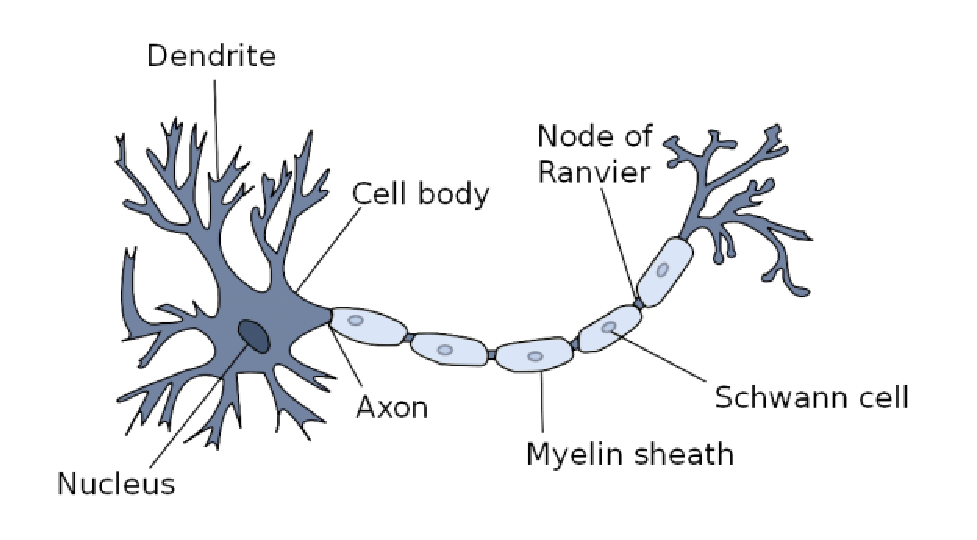
\includegraphics[scale = 0.5]{neuron.eps}
			
			\caption{}
			\label{fig:neuron}
		\end{figure}
		
		\begin{figure}[H]
			\center
			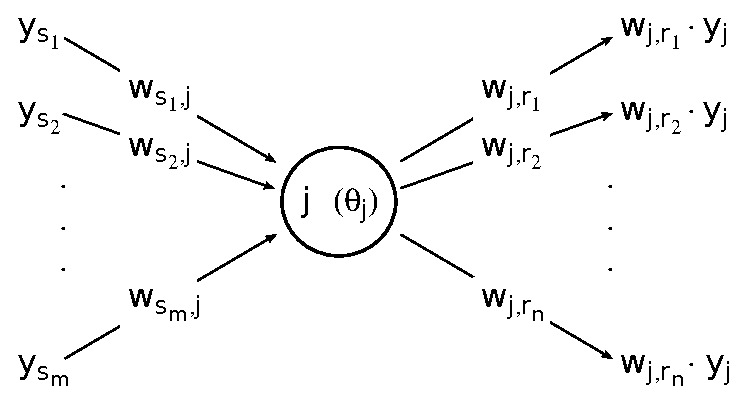
\includegraphics[scale = 0.7]{neural_model_ter.eps}
			
			\caption{}
			\label{fig:neural-model}
		\end{figure}
		
		\begin{figure}[H]
			\center
			\includegraphics[scale = 0.7]{neural_model_bias.eps}
			
			\caption{}
			\label{fig:neural-model-bias}
		\end{figure}
		
		\begin{figure}[H]
			\center
			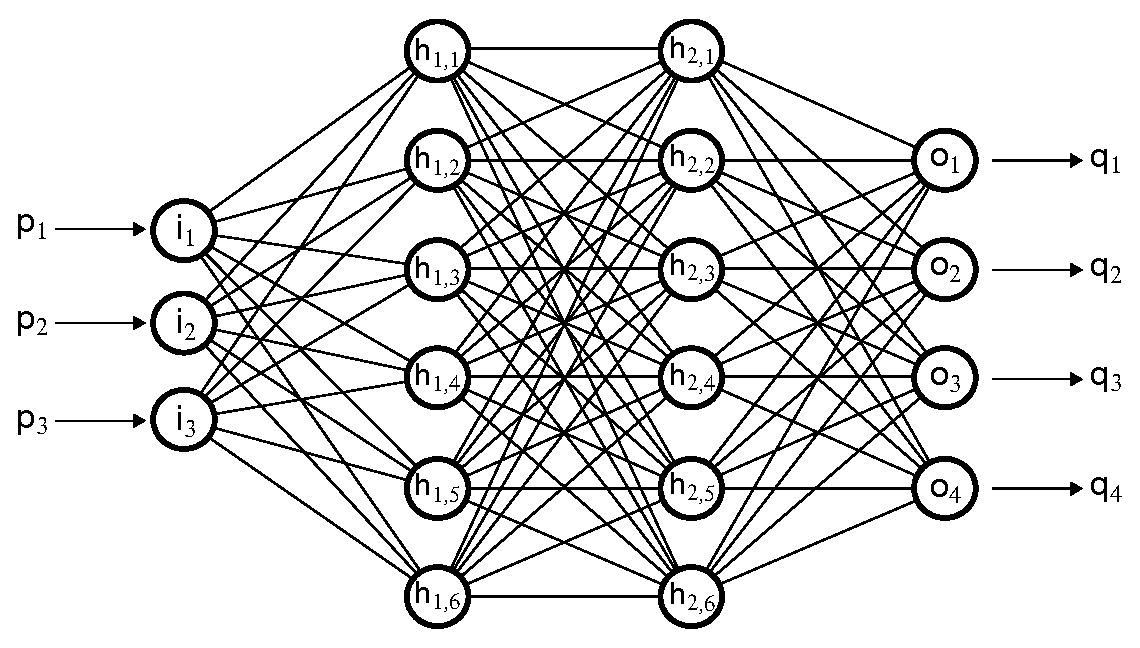
\includegraphics[scale = 0.6]{neural_network_bis.eps}
			
			\caption{}
			\label{fig:neural-network}
		\end{figure}
		
	 
		 
		 
		 

	\chapter{Reduced Basis method for nonlinear elliptic PDEs}
	\label{chapter:Reduced Basis method for nonlinear elliptic PDEs}
	
		In this chapter, we derive a Reduced Basis (RB) approximation for a parametrized Boundary Value problem (BVP) involving a possibly nonlinear elliptic Partial Differential Equation (PDE). As a convenient test case, the nonlinear Poisson equation in one and two spatial dimensions is considered, with the nonlinearity stemming from a solution-dependent viscosity. In the one-dimensional case, the parameters may characterize the viscosity itself, the forcing term, or the boundary conditions. On the contrary, in the two-dimensional framework we are concerned with a parameter-free PDE defined on a domain undergoing geometrical transformations. In the RB context, when dealing with shape variations one needs to introduce a parametric transformation, mapping the whole domain to a parameter-independent reference configuration, e.g. a unit square \cite{MN16}. For this aim, we refer to the boundary displacement-dependent transfinite map (BDD TM) proposed in \cite{JIR14}, building a volumetric parametrization given the boundary parametrization of the domain. 
		
		For the sake of numerical efficiency, the RB procedure is usually carried out within an offline-online framework. The \emph{offline} stage consists in generating the reduced basis out of an ensemble of \emph{snapshots}, i.e. high-fidelity numerical solutions to the BVP for different realizations of the parameters. In this thesis, the well-known Proper Orthogonal Decomposition (POD) technique is used, relying on the Finite Element (FE) method for the computation of the snapshots. Then, given new values for the parameters, in the \emph{online} phase one seeks an approximation to the high-fidelity solution in the reduced space, i.e. the linear space generated by the reduced basis. To retain the well-posedness of the problem, the system yielded by the FE method is projected onto the reduced space, thus enforcing the orthogonality to the reduced basis of the residual for each equation \cite{HRS15,MN16}. Hence, the computational cost associated with the \emph{resolution} of the \emph{reduced} model is \emph{independent} of the size of the original, large-scale model. 
		
		The whole procedure sketched so far is detailed in the following sections. Section \ref{} and \ref{} discuss the Finite Element method applied to the one- and two-dimensional Poisson equation, respectively. The Reduced Basis technique is described in Section \ref{}, while in the final Section \ref{} we present an alternative, Neural Network-based approach for the computation of the reduced solution, which represents the actual novelty of the proposed reduced order modeling algorithm.
		
	\section{Finite Element method for one-dimensional Poisson}
	\label{section:Finite Element method for one-dimensional Poisson}
		
		
	\begin{thebibliography}{50}
	
		\bibitem{Hag14}
		Hagan M. T., Demuth H. B., Beale M. H., De Jes\'us O. \emph{Neural Network Design, 2nd Edition}. eBook, 2014.
		
		\bibitem{Hay05}
		Haykin S. \emph{Neural Networks: A comprehensive foundation}. Prentice Hall, Upper Saddle River, NJ, 2004.
		
		\bibitem{Kri}
		Kriesel D. \emph{A Brief Introduction to Neural Networks}. \url{http://www.dkriesel.com/en/science/neural_networks}.
		
		\bibitem{Nie15}
		Nielsen M. A. \emph{Neural Networkd and Deep Learning}. Determination Press, 2015.
		
		\bibitem{SD}
		Stergiou C., Siganos D. \emph{Neural Networks}. \url{https://www.doc.ic.ac.uk/~nd/surprise_96/journal/vol4/cs11/report.html#Introduction to neural networks}.
		
	\end{thebibliography}	
	
\end{document}
